\section{Data preprocessing}
\label{sec:Data preprocessing} % 1 page
After collecting videos uploaded by participants to create a video data set, data preprocessing is the next process of adjusting the data to meet the research ethics requirements processing it into an input format suitable for the model data loader.
The encoding format of video recorded in the browser is WebP, a highly compressed video format developed by Google.
If the model data loader decodes the video data during the training process, it will consume lots of CPU during the decompression and anonymisation process.

An optimisation method is decoding the video into a sequence of pictures in the data preprocessing process to reduce the computational overhead in the training process.
An anonymous algorithm will be applied to each frame and save the results in picture format.
In this way, the data loader only needs to load the processed pictures during the training process.

According to research ethics requirements, the data preprocessing process will use an anonymisation algorithm to minimise the presence of facial details that might enable the identification of an individual.
The anonymisation algorithm cannot directly mask the face completely.
Because the facial information contains many features that help the model to classify activities, such as the direction of sight, the lips movement during speaking, etc.

The anonymisation algorithm should strike a balance between the complexity of implementation, performance, and the ability to keep research related facial features.
In the research, a simple two-step algorithm, namely feature masked face concealment, is used to extract the key facial features while covering the other facial areas.

The following two subsections will introduce the details of the two-step process in the anonymisation algorithm.
The first step is to find and locate faces in the video, and the second step is to extract facial feature points and perform masking on each frame.

\subsection{Face detection with Viola–Jones algorithm} % 1 page
\citet{viola2001rapid} proposed a fast object detection approach using Haar-like features, namely Viola–Jones algorithm, which extracts features from input images using a series of adjacent rectangular regions.
This operation is very similar to the convolution operation in convolutional neural networks.
However, the difference is that the proposed Haar Cascade uses predefined feature extraction kernels, such as edge features, line features, etc.
The classifier part uses AdaBoost algorithm, a famous Boosting method in ensemble learning, in which it trains many weak classifiers to form a more accurate strong classifier.

Currently, this algorithm is very mature and has been widely used in many studies.
For example, a previous study of virtual exam controller proposed by \citet{garg2020convolutional} was introduced early in the literature review section \ref{sec:Online exam security system}.
In this case, they use Haar Cascade Classifier to detect, tag, and identify the students face and using deep learning to apply exam constraints.

Technically, Haar Cascade Classifier use cascade structure to form multiple stages to classify face regions as shown in Figure \ref{fig:ext-haar-arch}.
This classifier has four vital features that enable it to be widely used in face detection tasks quickly, summarised by \citet{garg2020convolutional} as follows:

\begin{minipage}{\textwidth}
    \begin{minipage}{.4\textwidth}
        \begin{itemize}
            \item Using Haar-like features.
            \item Using the integral picture.
            \item Using AdaBoost learning.
            \item Using cascading classifiers.
        \end{itemize}
    \end{minipage}
    \begin{minipage}{.58\textwidth}
        \centering
        \captionsetup{type=figure}
        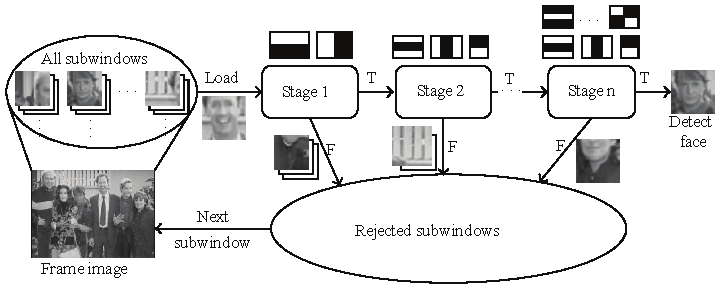
\includegraphics[width=\textwidth]{design/imgs/ext-haar-arch.pdf}
        \captionof{figure}{Haar Cascade structure \cite{kim2015system}}
        \label{fig:ext-haar-arch}
    \end{minipage}
\end{minipage}

OpenCV has provided a good implementation, cv::CascadeClassifier\footnote{cascadedetect.cpp: \url{https://github.com/opencv/opencv/tree/4.5.3/modules/objdetect/src}} and a variety of trained models\footnote{Available models: \url{https://github.com/opencv/opencv/tree/4.5.3/data/haarcascades}} for selection.
In addition, the API design for this module is clear and easy to use.
The trained model can be loaded through cv::CascadeClassifier::load method, and then cv::CascadeClassifier::detectMultiScale can be used to locate the face positions in the input image and return the result of faces in the format of rectangular areas.

To summary, this Haar Cascade object detection method is suitable for real-time face detection on mobile devices with the advantage of requiring a small amount of calculation. 
Therefore, this research will use this method to perform the face detection procedure in the anonymisation algorithm.

\subsection{Face landmark extraction and face concealment} % 1 page
As mentioned above, after obtaining the position of faces from the input video, it also needs to extract face landmark points and overlay them on the top after masking face details.

A highly efficient and accurate face alignment algorithm was proposed by \citet{ren2014face} in 2014.
This research still uses classic machine learning methods for low computation complexity by using a combination of random forest and global linear regression to regress key points of facial features.
It learns the local binary features of each key point through random forest, then combines the features and uses linear regression to obtain the key points.

\begin{figure}[!ht]
    \centering
    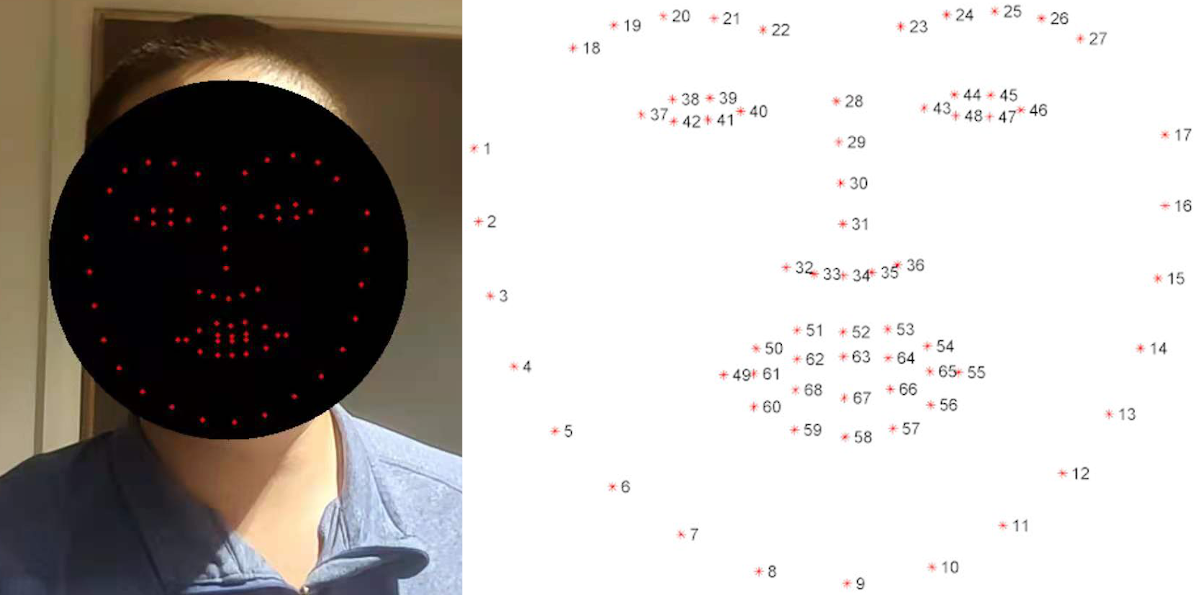
\includegraphics[width=\textwidth]{design/imgs/3-face-landmark.png}
    \caption{Landmark masked face concealment and face landmark schematic}
    \label{fig:3-face-landmark}
\end{figure}

The left picture in Figure \ref{fig:3-face-landmark} illustrates an exemplar face image (anonymised result) with landmark masked face concealment applied.


Local Binary Features (LBF)

\citet{casado2021real}

In OpenCV, cv::FacemarkLBF